% Build from this directory: tectonic --keep-logs result_collation.tex
% Numerical source: results/completed_runs_2026-11-17/{audits,tables}/.
% This document reports completed runs; it does not initiate new fitting.
\documentclass[11pt,a4paper]{article}
\usepackage[margin=2.2cm]{geometry}
\usepackage[T1]{fontenc}
\usepackage{lmodern}
\usepackage{microtype}
\usepackage{amsmath,amssymb}
\usepackage{graphicx}
\usepackage{booktabs,longtable,array}
\usepackage{caption}
\usepackage{placeins}
\usepackage[numbers,sort&compress]{natbib}
\usepackage{xurl}
\usepackage[hidelinks]{hyperref}
\hypersetup{pdftitle={Synthetic results and discussion: completed notebook runs},
  pdfsubject={Completed synthetic validation, 17 November 2026}}
\newcommand{\cgc}{c-GC}
\newcommand{\cgcs}{c-GC$^{*}$}
\newcommand{\fastcgc}{fastC-GC}
\newcommand{\fastcgcs}{fastC-GC$^{*}$}
\newcommand{\artifacts}{results/completed_runs_2026-11-17}
\graphicspath{{results/completed_runs_2026-11-17/figures/}}
\captionsetup{font=small,labelfont=bf}
\setlength{\emergencystretch}{2em}
\setlength{\parskip}{0.35em}
\setlength{\parindent}{0pt}
\setcounter{tocdepth}{1}

\title{Synthetic results and discussion\\
  \large Collation of completed notebooks 00--06}
\author{Effectome-to-behavior project\\\small Research results report}
\date{17 November 2026}

\begin{document}
\maketitle

\begin{abstract}
The completed synthetic runs establish correct native graph recovery in a bounded
sanity control, but do not establish reliable transition-driver recovery across
the main benchmark. All 24 chain/null fits recover the expected support, all 48
framework-smoke fits complete, and all 560 method/recording entries in the frozen
driver study are available. Framework prediction gains have no multiplicity-adjusted
support across 16 contrasts. Every method fails the frozen driver criteria, with
false nominations in 20--50 of 60 null seeds. A revised, graph-constrained nonlinear
mechanism readout provides a favorable operating case: on one existing development
seed, increasing discovery history from 256 to 1,024 samples raises driver top-$k$
recall from $1/6$ to 1 for all four native methods and reduces intervention-effect
mean absolute error by 98.69\%. This result motivates independent replication and
nomination calibration. It does not overturn the earlier failure, validate the
partially observed setting, or add new independent confirmation.
\end{abstract}

\tableofcontents

\section{Scope and current status}
\label{sec:scope}

This report collates the completed \texttt{faster-machine-03} artifacts from
synthetic notebooks 00--06. Every code cell in the seven saved notebooks has an
execution count, and none contains a saved execution-error output. The numerical
evidence, exact notebook copies, source reports, figures, citation audit and
provenance are preserved in \path{results/completed_runs_2026-11-17/}.
The analysis performs no new fits. Graph-similarity experiments on the separate
feature branch, including notebook 07, are outside the present evidence.

The central question is whether estimated effectomes help predict future
transitions and recover intervention-defined drivers. The studies answer different
parts of that question. Native graph sanity tests support discovery in a simple
control; graph augmentation tests incremental prediction; the frozen driver study
compares feature-omission scores with structural intervention truth; and the revised
mechanism diagnostic estimates disconnection effects through fitted transition
equations. A successful result at one stage does not automatically validate the
later stages.

\begin{table}[htbp]
\centering
\small
\caption{Execution inventory. Entries count completed method fits or evaluation
lanes, not independent replications. The mechanism reports include known-support
and empty-support controls. The same development seed is reused in all three
mechanism panels.}
\label{tab:inventory}
\begin{tabular}{@{}p{4.2cm}rp{8.1cm}@{}}
\toprule
Stage & Available/planned & Independent unit and scope \\
\midrule
Native chain/null sanity & 24/24 & Three raw-process seeds per condition; four methods. \\
Shared transition example & 4/4 & One recording, raw seed 42. \\
Framework smoke & 48/48 & Three seeds for each of four specifications; 12 cells. \\
Frozen driver benchmark & 560/560 & 20 seeds for each non-null scenario and 60 null seeds; 140 cells. \\
Mechanism smoke & 12/12 & One seed per driver/null scenario; six lanes. \\
Mechanism, history 256 & 12/12 & Existing seed 20; paired with history 1,024. \\
Mechanism, history 1,024 & 12/12 & Existing seed 20; includes both support controls. \\
\bottomrule
\end{tabular}
\end{table}

Rerunning the same raw-process seeds is a reproducibility exercise. The present
driver and mechanism reruns reuse the earlier study seeds and must not be counted
as new independent confirmation. Likewise, methods, directions, neurons, windows,
trials and Monte Carlo rollouts do not increase the number of independent process
seeds. The four methods are related variants within the GC discovery family.

\section{Evaluation definitions and statistical reporting}
\label{sec:definitions}

\subsection{Native graph estimates and the two attribution questions}

The conventional \cgc/\cgcs{} and fast \fastcgc/\fastcgcs{} implementations are
imported upstream methods \citep{adedayo2025cgc,adedayo2026fastcgc}. The present
adapters expose unsigned binary positive-lag cross-neuron support. They do not
return interaction signs, fitted structural coefficients or complete intervention
distributions. Self-edges and zero-lag edges are excluded from the reported native
support.

Predictive gain is defined as
\begin{equation}
  G = \mathcal{L}_{\mathrm{activity}}-
      \mathcal{L}_{\mathrm{activity+graph}},
\end{equation}
where $\mathcal{L}$ is held-out transition log loss in nats. Positive gain favors
graph augmentation. The old attribution score is the increase in loss after
refitting without a neuron's outgoing graph-feature block. Its measured activity
and the population/manifold variables remain in the predictor. The score therefore
measures conditional predictive contribution, consistent with the distinction
between full and reduced predictive models \citep{williamson2023importance}.

Structural disconnection asks a different question. The simulator removes a
candidate's outgoing cross-neuron influence from every future update, retaining
its own equation and self-history. For a candidate set $S$, the target quantity is
the probability reduction
\begin{equation}
  \Delta(S)=P(Y=1\mid h)-
  P\!\left(Y=1\mid h;\ \text{outgoing influence of }S\text{ disconnected}\right),
  \label{eq:effect}
\end{equation}
conditional on an evaluation history $h$. Intervening on structural assignments
requires more information than a graph mask alone \citep{pearl2010causalinference}.
Conditional predictive contribution and structural influence need not agree when
other observed variables retain information about a source.

\subsection{Replication, intervals and decision rules}

The framework summaries use independent raw-seed gains: means, sample standard
deviations and the existing 2,000-resample percentile intervals for seed means
\citep{efron1979bootstrap}. With three seeds per specification, these intervals
have sparse empirical support and unstable coverage. The prespecified two-sided
exact sign tests exclude only exact-zero gains; their implementation uses the
binomial test \citep{scipyBinomtest}. Holm correction covers the complete family
of 16 framework contrasts \citep{holm1979sequential}. This test concerns the sign
tendency of gain, not a test of its mean magnitude or equivalence.

For the driver benchmark, the two directions are averaged within each independent
seed before descriptive aggregation. A null seed contributes one Bernoulli event:
whether any false candidate or group is nominated in either direction. If $k$ of
$n$ independent null seeds have that event, the one-sided exact 95\% upper bound is
\begin{equation}
 U_{0.95}(k,n)=
 \begin{cases}
  \operatorname{BetaQuantile}(0.95;k+1,n-k), & k<n,\\
  1, & k=n.
 \end{cases}
 \label{eq:nullbound}
\end{equation}
This is binomial-tail inversion \citep{clopper1934confidence}. Coverage is per
method and assumes independent seeds and a fixed nomination rule. It is not a
posterior probability, neuron-level false-discovery rate, or simultaneous
guarantee across all methods. The one-seed mechanism comparison receives no
between-seed standard deviation, process-level confidence interval or $p$-value.

\section{Generating-process controls and native graph sanity}
\label{sec:controls}

\subsection{Designed correspondence and mismatch}

Notebook 00 checks four designed scenarios at raw seed 42, each with 1,536 samples.
The one-to-one and matched-marginals scenarios contain two true circuit regimes;
the fixed-circuit and stationary controls contain one. In the matched-marginals
construction, the circuits have distinct coefficient matrices, zero stationary
means and unit stationary covariance diagonals. The saved covariance-equation
residual is $2.22\times10^{-16}$ for each circuit. Thus distinct designed dynamics
can share stationary marginal distributions. The metadata flag
\texttt{matched\_stationary\_marginals} denotes that construction; a false flag in
the other scenarios is not an execution failure.

Notebook 03 uses the true generating regime and a fixed activity-sign partition,
$A=\mathbf{1}\{X_0\geq0\}$, on 384 held-out samples per scenario. These labels are
separate from inferred graph states and the learned manifold in notebook 02.
Table~\ref{tab:designed} shows the expected contrast: a tight designed association
in the one-to-one example, weak association in the matched-marginals example, and
activity variation despite a constant circuit label in the controls.

\begin{table}[htbp]
\centering
\caption{Descriptive generating-process correspondence, in nats. $C$ is the true
circuit regime and $A$ is the fixed activity-sign bin. One seed is used throughout;
zero $H(C\mid A)$ for a constant circuit is automatic.}
\label{tab:designed}
\begin{tabular}{@{}lrr@{}}
\toprule
Scenario & $H(C\mid A)$ & $H(A\mid C)$ \\
\midrule
One-to-one & 0.076936 & 0.080485 \\
Matched marginals & 0.636344 & 0.692313 \\
Fixed circuit & 0.000000 & 0.693134 \\
Stationary & 0.000000 & 0.692279 \\
\bottomrule
\end{tabular}
\end{table}

The 20 circular-shift controls per scenario reuse the same recording. They are
descriptive surrogates, not 20 independent process seeds. These constructive
examples demonstrate possible correspondence and mismatch; they do not validate
discovered neural regimes or establish biological circuit equivalence.

\subsection{Native chain and null recovery}

Notebook 01 evaluates four methods on a four-neuron chain/null control over seeds
0--2. All 24 fits are available and recover the exact expected support. Each chain
fit identifies the two planted edges, $0\to1$ and $1\to2$, without false edges;
neuron 3 is disconnected. Each null fit selects no cross-neuron edges.

This is a positive technical control for the discovery adapters under the tested
settings. Precision/recall and empty-graph Jaccard can be undefined when their
denominators are zero; such values do not imply an unavailable fit. Three null
seeds are also insufficient to establish a 5\% false-nomination bound for a later
driver-ranking procedure. Native edge recovery and driver nomination are separate
outcomes with different denominators and decision rules.

\section{Shared prediction example and framework smoke}
\label{sec:prediction}

\subsection{One matched-marginals recording}

Notebook 02 compares the four methods on common training-owned manifold/event
definitions, with 164 training origins and 60 held-out origins, including 30 exits.
The activity-only baseline log loss is 1.393110 nats. Both fast variants improve
that value in this recording, while both conventional variants worsen it
(Table~\ref{tab:shared}). A single raw seed cannot support a general method ranking.

\begin{table}[htbp]
\centering
\caption{Shared example, seed 42. Gain is baseline minus augmented log loss.
The last column counts occupied held-out graph states, not requested clusters.}
\label{tab:shared}
\begin{tabular}{@{}lrrr@{}}
\toprule
Method & Augmented log loss & Gain (nats) & Occupied states \\
\midrule
\cgc & 1.482440 & $-0.089330$ & 2 \\
\cgcs & 1.463098 & $-0.069988$ & 2 \\
\fastcgc & 1.381873 & $+0.011236$ & 1 \\
\fastcgcs & 1.362782 & $+0.030328$ & 1 \\
\bottomrule
\end{tabular}
\end{table}

Both fast methods occupy only one held-out graph state despite requesting two
states during training. A zero conditional entropy of effectome code given
manifold state can therefore result from a constant graph code. It is not evidence
of informative correspondence. More fundamentally, unsigned support cannot encode
a switch that changes interaction signs while preserving edge presence. Any
comparison based solely on that support inherits this representation limit.

\subsection{Repeated framework evaluation}

Notebook 04 completes its separate smoke protocol: four scenarios, three seeds
each, 12 cells and 48 method runs. The distinct manuscript matrix of 7,680 cells
and 30,720 method entries was not executed by this smoke run. In the two switching
scenarios, every mean graph-augmentation gain is negative
(Table~\ref{tab:framework}). Small positive means in the stationary control do not
survive the statistical comparison. All 16 Holm-adjusted sign-test $p$-values equal
1, and all 1,632 exported attribution rows retain their unvalidated status.

\begin{table}[htbp]
\centering
\small
\setlength{\tabcolsep}{4pt}
\caption{All framework-smoke contrasts. Each row uses three raw-process seeds.
Values are nats; SD is the sample SD. The existing percentile-bootstrap 95\%
intervals are descriptive and unstable at this seed count. All Holm-adjusted
$p$-values are 1.000. Rounded zeros can include floating-point residuals.}
\label{tab:framework}
\begin{tabular}{@{}llrr@{}}
\toprule
Scenario & Method & Mean gain $\pm$ SD & Descriptive 95\% interval \\
\midrule
One-to-one & \cgc & $-0.372170 \pm 0.407253$ & $[-0.798940,\ +0.012257]$ \\
 & \cgcs & $-0.038429 \pm 0.089100$ & $[-0.137601,\ +0.034872]$ \\
 & \fastcgc & $-0.073192 \pm 0.117622$ & $[-0.208869,\ +0.000000]$ \\
 & \fastcgcs & $-0.005182 \pm 0.008976$ & $[-0.015547,\ +0.000000]$ \\
\midrule
Matched marginals & \cgc & $-0.165287 \pm 0.142596$ & $[-0.251147,\ -0.000683]$ \\
 & \cgcs & $-0.058948 \pm 0.039813$ & $[-0.104881,\ -0.034337]$ \\
 & \fastcgc & $-0.024108 \pm 0.038167$ & $[-0.059777,\ +0.016143]$ \\
 & \fastcgcs & $-0.021977 \pm 0.019299$ & $[-0.036162,\ +0.000000]$ \\
\midrule
Fixed circuit & \cgc & $-0.003189 \pm 0.002491$ & $[-0.004706,\ -0.000314]$ \\
 & \cgcs & $-0.000406 \pm 0.000702$ & $[-0.001217,\ +0.000000]$ \\
 & \fastcgc & $-0.001878 \pm 0.002454$ & $[-0.004706,\ -0.000314]$ \\
 & \fastcgcs & $+0.000000 \pm 0.000000$ & $[+0.000000,\ +0.000000]$ \\
\midrule
Stationary & \cgc & $-0.027961 \pm 0.042584$ & $[-0.073176,\ +0.011382]$ \\
 & \cgcs & $+0.000755 \pm 0.045046$ & $[-0.051224,\ +0.028394]$ \\
 & \fastcgc & $+0.006930 \pm 0.012003$ & $[-0.000000,\ +0.020790]$ \\
 & \fastcgcs & $+0.000000 \pm 0.000000$ & $[-0.000000,\ +0.000000]$ \\
\bottomrule
\end{tabular}
\end{table}

\begin{figure}[htbp]
\centering
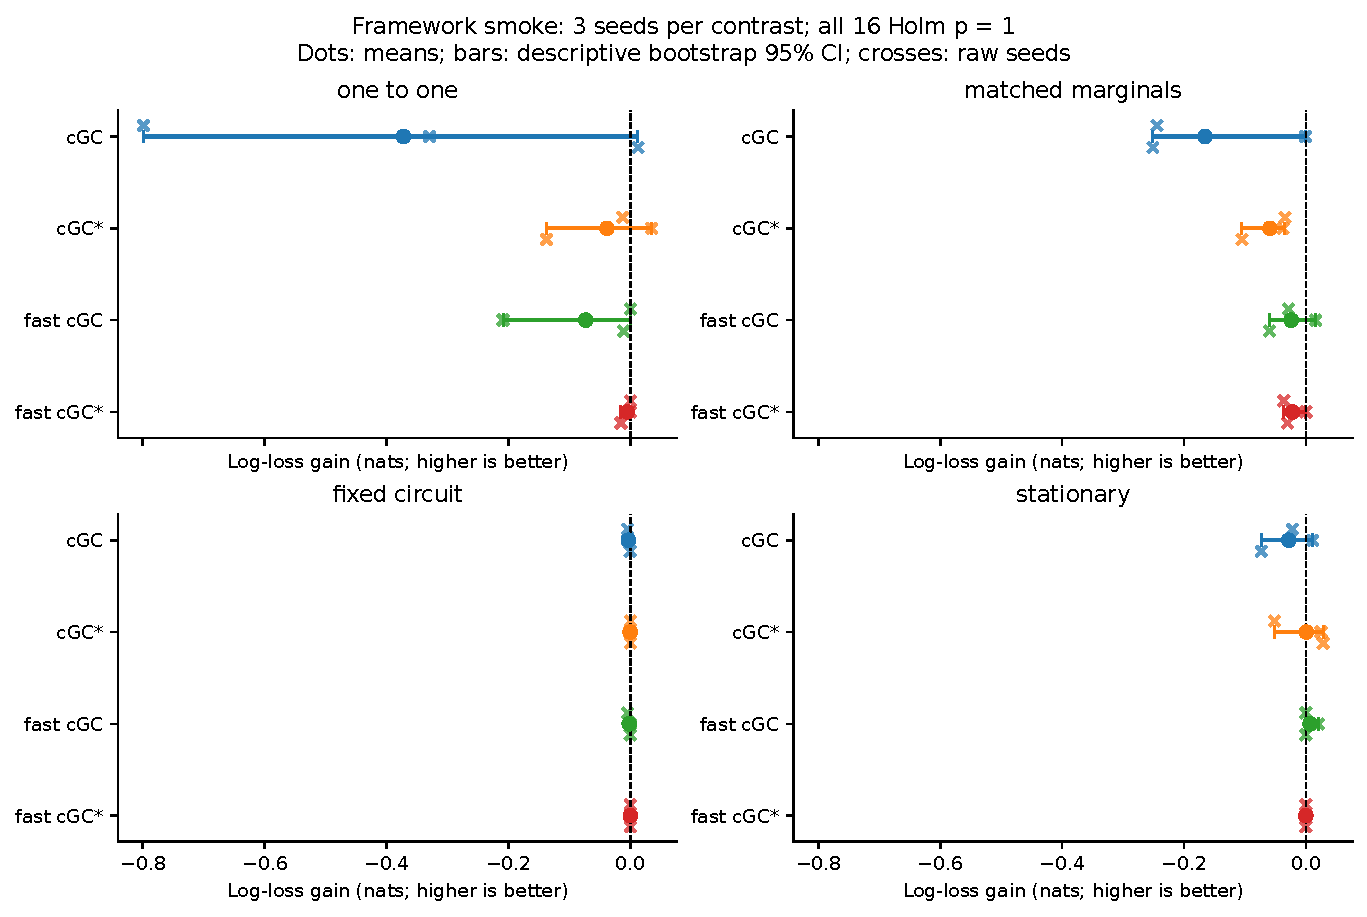
\includegraphics[width=\linewidth]{01-framework-gains.pdf}
\caption{Framework-smoke prediction gains. Crosses are independent seed gains;
dots and bars are means and existing percentile-bootstrap 95\% intervals. The
zero line marks equal held-out log loss. The common scale exposes the adverse
one-to-one conventional result and the lack of consistent improvement across
controls. All four methods are evaluated on paired input cells.}
\label{fig:framework}
\end{figure}

Prediction includes mixed-regime histories. Structural graph recovery is instead
restricted to pure-history origins: 33 of 60 held-out origins in each switching
cell, 32 of 32 in the fixed-circuit control and 60 of 60 in the stationary control.
Those different denominators must be retained. Near-$10^{-14}$ gains can count as
positive in the existing exact-sign implementation, but have no substantive
predictive interpretation. The small bootstrap intervals and the sign tests answer
different questions; neither warrants a superiority or equivalence claim here.

\FloatBarrier
\section{Frozen transition-driver benchmark}
\label{sec:driver}

\subsection{Execution and eligibility are complete}

Notebook 05 evaluates single-driver, redundant-group, correlated-bystander, null
and hidden-confounder scenarios. The four non-null scenarios each use seeds
300--319; the null uses seeds 400--459. All 140 scenario/seed cells and 560 method
entries complete. All 1,120 directional rows are available and eligible. Directional
origins range from 24 to 40, event counts from 10 to 27, endpoint alignment from
0.80 to 1.00, and source-well purity is 1.00. The failures therefore cannot be
attributed to unavailable conventional methods or insufficient eligibility counts.

The frozen gates require availability at least 0.90, nonnegative mean predictive
gain, and single-driver/bystander top-$k$ recall at least 0.75. The redundant-group
criterion requires a group-win fraction at least 0.75 and positive group advantage.
The null one-sided upper bound must be at most 0.05. Hidden confounding is a
diagnostic scenario rather than a required pass. The profile name
\texttt{confirmatory} denotes the internal frozen study configuration; it does not
mean external preregistration or successful confirmation.

\subsection{Every method fails the declared recovery and null criteria}

All recovery means are below 0.75 (Table~\ref{tab:recovery}). Single-driver recall
ranges from 0.025 to 0.325 and correlated-bystander recall from 0.025 to 0.200.
Redundant-group wins range from 0.150 to 0.325. Individual top-$k$ recovery is
undefined for the redundant scenario under the frozen intervention threshold:
individual true effects are small, while the joint effect is substantial. The
group criterion is therefore the relevant prespecified outcome for that scenario.

\begin{table}[htbp]
\centering
\small
\caption{Driver-recovery means $\pm$ sample SD across 20 independent seeds,
averaging the two directions within seed. All three acceptance minima are 0.75;
the third column of outcomes is a group-win fraction rather than individual
top-$k$ recall. Every method fails overall acceptance.}
\label{tab:recovery}
\begin{tabular}{@{}lrrr@{}}
\toprule
Method & Single-driver recall & Bystander recall & Redundant-group win \\
\midrule
\cgc & $0.325 \pm 0.373$ & $0.050 \pm 0.154$ & $0.200 \pm 0.251$ \\
\cgcs & $0.150 \pm 0.235$ & $0.025 \pm 0.112$ & $0.325 \pm 0.406$ \\
\fastcgc & $0.200 \pm 0.299$ & $0.200 \pm 0.251$ & $0.150 \pm 0.328$ \\
\fastcgcs & $0.025 \pm 0.112$ & $0.075 \pm 0.183$ & $0.225 \pm 0.302$ \\
\bottomrule
\end{tabular}
\end{table}

Gold neurons require paired simulator probability reduction at least 0.10 per
direction; $k$ is the number of gold neurons in that direction. Operational
nomination requires an omission score strictly greater than 0.01 nats.
The null results show substantial false nomination rather than merely an
underpowered upper bound: the observed event rates range from 0.333333 to 0.833333
(Table~\ref{tab:null}). Every upper bound exceeds the 0.05 gate. Gold-sized top-$k$
ranking is distinct from operational nomination. Better ranking alone would not repair this specificity
failure.

\begin{table}[htbp]
\centering
\caption{Whole-seed null false-nomination events. The bound is one-sided exact
95\% coverage per method, over 60 independent null seeds. The event includes any
false candidate/group in either direction.}
\label{tab:null}
\begin{tabular}{@{}lrrr@{}}
\toprule
Method & False-event seeds & Observed rate & Upper bound \\
\midrule
\cgc & 50/60 & 0.833333 & 0.906693 \\
\cgcs & 20/60 & 0.333333 & 0.446466 \\
\fastcgc & 42/60 & 0.700000 & 0.796294 \\
\fastcgcs & 24/60 & 0.400000 & 0.514351 \\
\bottomrule
\end{tabular}
\end{table}

Every method also has negative mean predictive gain in each required positive
scenario (Appendix~\ref{app:drivergains}). Thus the failed ranking is accompanied
by failed incremental prediction. All redundant-group mean advantages are negative.
Figure~\ref{fig:driver} displays the recovery and null gates together; descriptive
intervals do not replace the frozen acceptance algorithm.

\begin{figure}[htbp]
\centering
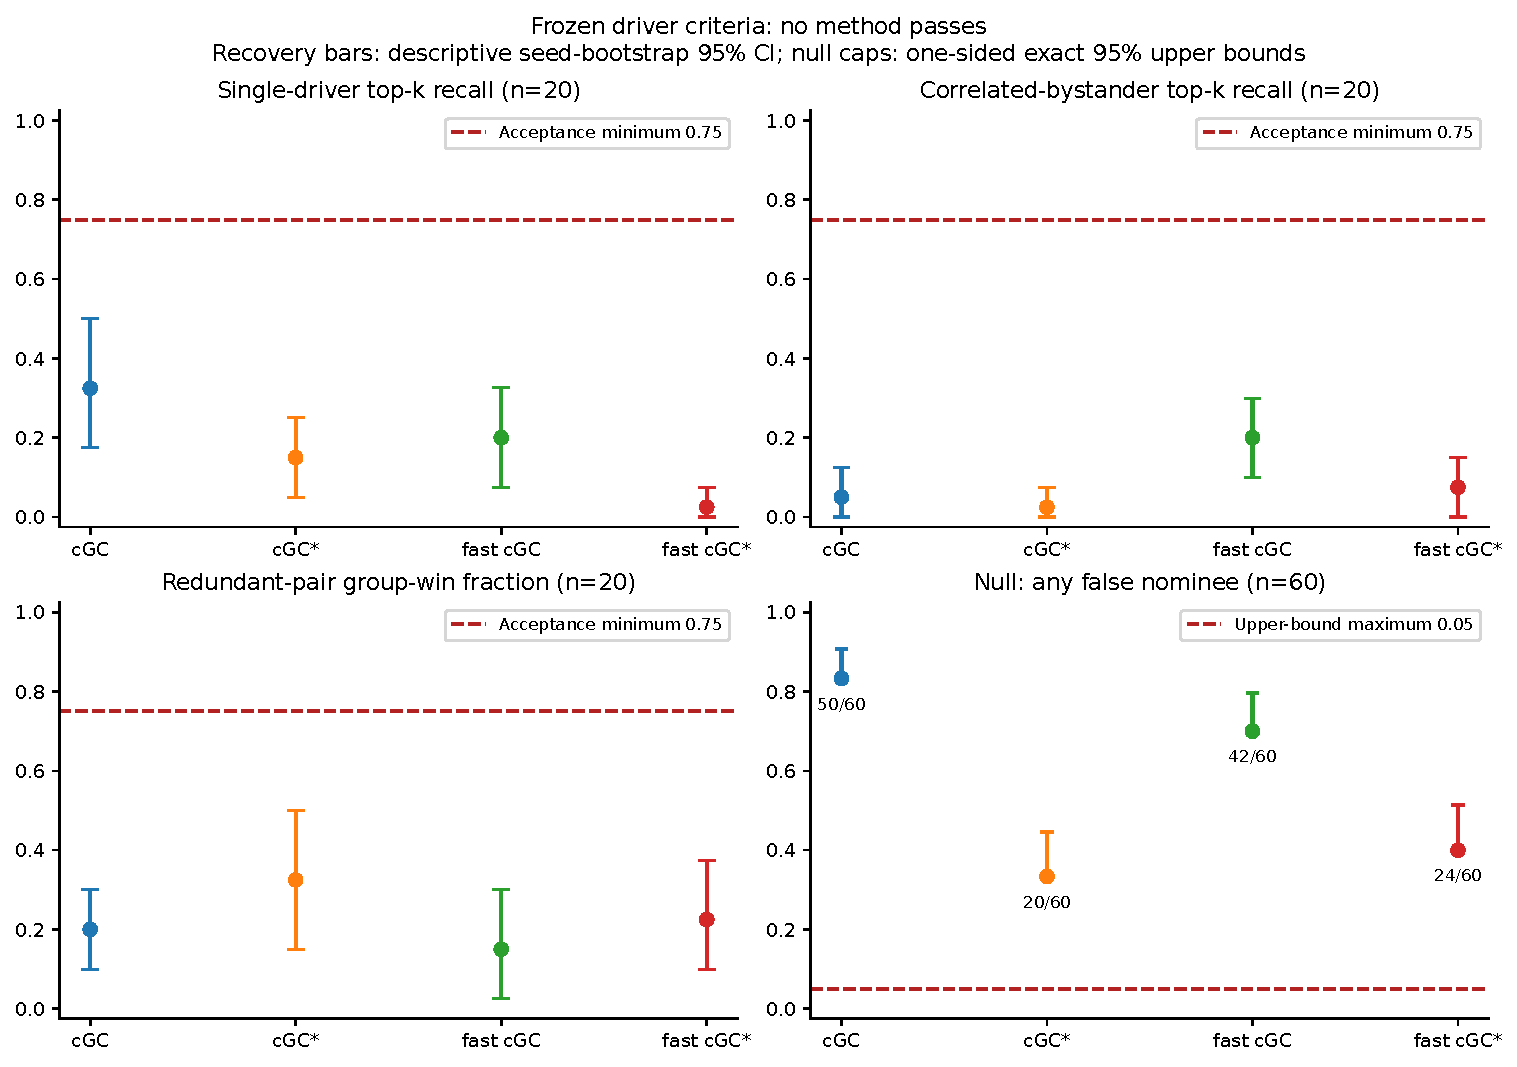
\includegraphics[width=\linewidth]{02-driver-gates.pdf}
\caption{Frozen driver benchmark: no method passes. Recovery points average
within-seed directions over 20 seeds; bars show stored descriptive seed-bootstrap
95\% intervals. Null points show the fraction of 60 seeds with any false nominee;
caps show one-sided exact 95\% upper bounds. Dashed lines mark the 0.75 recovery
minimum and 0.05 null-bound maximum.}
\label{fig:driver}
\end{figure}

\FloatBarrier
\section{Revised graph-constrained mechanism diagnostic}
\label{sec:mechanism}

\subsection{What changed and why}

The revised readout fits structural transition equations so that estimated
outgoing disconnections and simulator truth target the same operation. The favorable
control is fully observed, has six neurons, and uses additive nonlinear lag-one
updates of the form
\begin{equation}
 X_j(t+1)=b_j+a_jX_j(t)+
 \sum_{i\ne j}w_{ij}\tanh\!\left(X_i(t)\right)+\epsilon_j(t+1).
 \label{eq:scm}
\end{equation}
Known or estimated support constrains which cross-neuron terms are fitted.
Coefficients are learned with ridge regression \citep{hoerl1970ridge} using the
declared basis. This is a downstream transition readout; its coefficients are not
native CSL edge weights. Additive-noise models motivate explicit structural
assumptions \citep{peters2014additive}, but their identifiability results do not
automatically establish identifiability of this time-series implementation.

The diagnostic has six lanes: known support, empty support and four native support
estimates. Only the known-support lane receives the simulator's adjacency mask.
All learned lanes estimate their own coefficients and innovation scales. Discovery
uses inner-training trials 0--8; trials 9--11 are reserved for penalty/noise
selection; final mechanism fitting uses the outer training trials with fixed
support. Trials 12--23 are held out for evaluation. This separation limits model
selection bias \citep{cawley2010overfitting}. No histories are concatenated across
trial boundaries.

Factual and disconnected rollouts share innovations. The endpoint is an observed
coordinate fixed by the control design, and each evaluation uses 256 rollouts.
Effect MAE compares estimated and oracle probability reductions. Factual Brier
scores predicted probabilities against observed binary transition events; it is a
different outcome. The effect and nomination cutoffs in this development control
are 0.10 probability units. They are not a calibrated replacement for the old
0.01-nat omission cutoff.

\subsection{Short histories fail; longer histories recover the operating case}

All three reports complete both driver/null cells and all 12 method/control lanes,
for 36 available lanes in total. Each scenario still has only one existing raw
seed, 20. The regular smoke panel has trial length 320 and discovery history 256.
The controlled history comparison uses trial length 1,152 for both histories, so
full mechanism fitting data, evaluation origins, oracle effects and rollout noise
remain identical. Its only intended change is discovery-history length.

Table~\ref{tab:mechanism} retains every driver lane. In the paired 256-sample panel,
each native method has top-$k$ recall $1/6$, effect MAE 0.140055339 and factual Brier
0.717281342. At 1,024 samples, each native lane has recall 1, effect MAE 0.001831055
and Brier 0.087547302, matching the known-support control on this input. Empty
support retains recall $1/6$ and high error. The $1/6$ values are expected recall
under the implemented tie-aware score for an all-zero ranking, not evidence that
one of six independent experiments succeeded.

\begin{table}[htbp]
\centering
\small
\setlength{\tabcolsep}{4pt}
\caption{All driver-scenario mechanism lanes, one existing seed per panel.
Top-$k$ recall averages eligible directions; effect MAE and factual Brier are
lower-is-better. Support recall concerns the full cross-neuron graph. Smoke uses
different recordings from the paired-history panels and is not a controlled
history contrast. Known and empty support are explicit diagnostic controls.}
\label{tab:mechanism}
\begin{tabular}{@{}llrrrr@{}}
\toprule
Panel & Method & Top-$k$ & Effect MAE & Brier & Support recall \\
\midrule
Smoke & Known support & 1.000000 & 0.003011068 & 0.075078328 & 1.000 \\
 & Empty support & 0.166667 & 0.146972656 & 0.795562744 & 0.000 \\
 & \cgc & 0.166667 & 0.146972656 & 0.795562744 & 0.500 \\
 & \cgcs & 0.500000 & 0.087076823 & 0.406508128 & 0.750 \\
 & \fastcgc & 0.166667 & 0.146972656 & 0.795562744 & 0.500 \\
 & \fastcgcs & 0.166667 & 0.146972656 & 0.795562744 & 0.500 \\
\midrule
History 256 & Known support & 1.000000 & 0.001831055 & 0.087547302 & 1.000 \\
 & Empty support & 0.166667 & 0.140055339 & 0.717281342 & 0.000 \\
 & \cgc & 0.166667 & 0.140055339 & 0.717281342 & 0.500 \\
 & \cgcs & 0.166667 & 0.140055339 & 0.717281342 & 0.500 \\
 & \fastcgc & 0.166667 & 0.140055339 & 0.717281342 & 0.500 \\
 & \fastcgcs & 0.166667 & 0.140055339 & 0.717281342 & 0.500 \\
\midrule
History 1,024 & Known support & 1.000000 & 0.001831055 & 0.087547302 & 1.000 \\
 & Empty support & 0.166667 & 0.140055339 & 0.717281342 & 0.000 \\
 & \cgc & 1.000000 & 0.001831055 & 0.087547302 & 1.000 \\
 & \cgcs & 1.000000 & 0.001831055 & 0.087547302 & 1.000 \\
 & \fastcgc & 1.000000 & 0.001831055 & 0.087547302 & 1.000 \\
 & \fastcgcs & 1.000000 & 0.001831055 & 0.087547302 & 1.000 \\
\bottomrule
\end{tabular}
\end{table}

For each native method, the paired change is $+0.833333$ top-$k$ recall,
$-0.138224284$ effect MAE (98.6926\% reduction), and $-0.629734039$ Brier.
At history 256, discovery counts for endpoint edges $0\to5$ and $1\to5$ are
$(4,3)$, $(1,3)$, $(1,0)$ and $(1,0)$ across the four native methods, each out of
nine inner-training histories. All are below the five-of-nine selection quorum.
At history 1,024, every method detects each endpoint edge in all nine histories.
This provides a direct support-level explanation for the paired contrast in this
input. It does not establish a general sample-complexity law or isolate the cause
of failure in the older partially observed generator.

\begin{figure}[htbp]
\centering
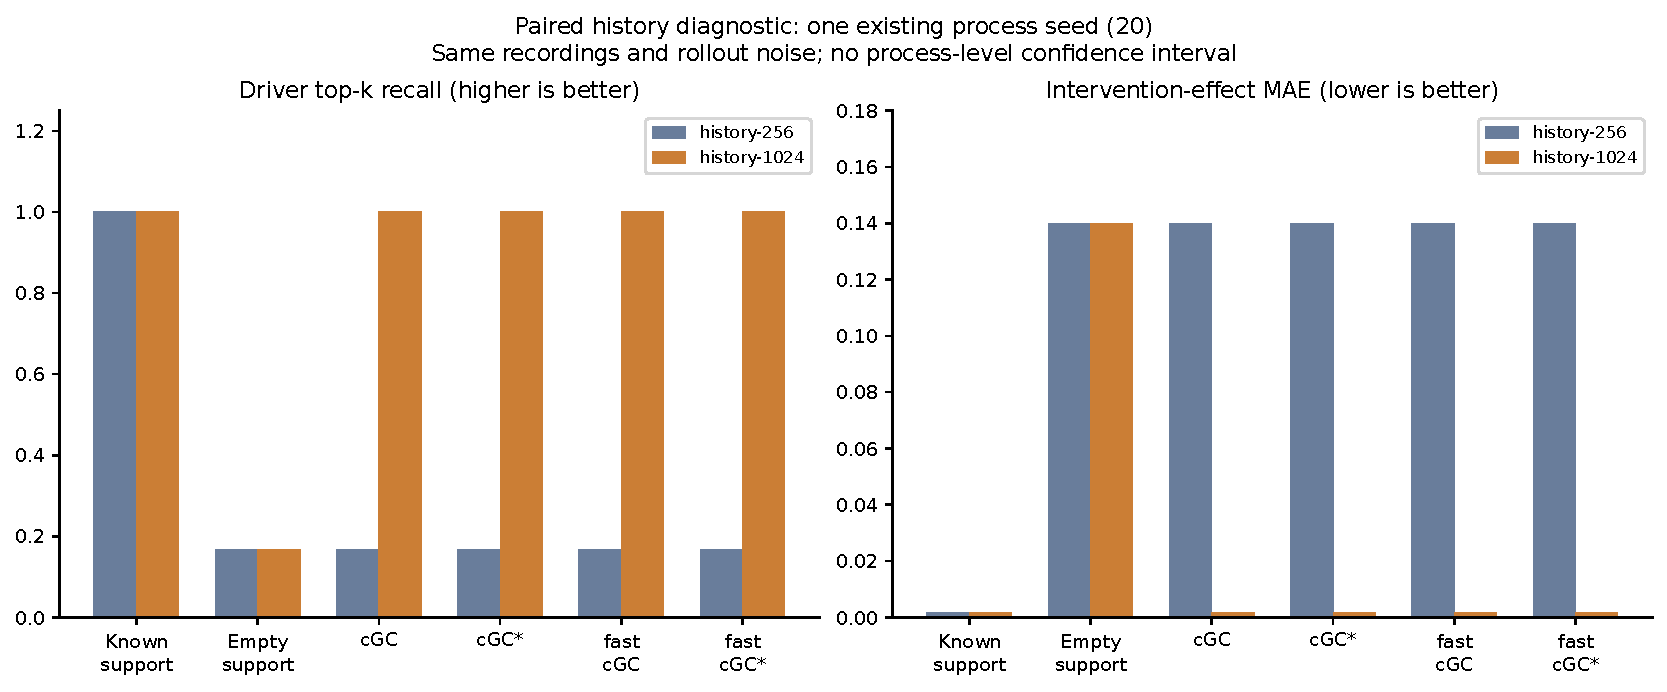
\includegraphics[width=\linewidth]{03-mechanism-history.pdf}
\caption{Paired discovery-history diagnostic on existing seed 20. Each pair of
bars uses identical full training data, held-out origins, oracle probabilities and
rollout noise. Longer native discovery histories recover the known-support
operating case, while empty support remains ineffective. No error bars or
process-level significance claim are justified by this one-seed comparison.}
\label{fig:mechanism}
\end{figure}

All mechanism null lanes report zero effect MAE and no false nomination in one
null seed. Equation~\eqref{eq:nullbound} gives an upper bound of 0.95 for zero of
one, not evidence of 5\% specificity. The three panels reuse the seed and cannot
be pooled into three independent null observations. No process-level confidence
interval or $p$-value is estimable for the reported history improvement.

\FloatBarrier
\section{Discussion}
\label{sec:discussion}

\subsection{What the findings currently establish}

The work now has a verified computational path and a bounded positive scientific
result. Native discovery recovers simple chain/null graphs, and the revised
readout learns accurate intervention effects when support is known. With sufficient
discovery history, all four native lanes reproduce that operating case on the
same development input. The empty-support failure and short-history failure make
the mechanism result more informative than a standalone favorable score: they
show which support condition changes the outcome within this control.

The larger benchmark supplies a clear negative result. All planned runs are
available, eligibility counts are adequate, recovery gates fail, predictive gains
are negative, and null false nominations are frequent. These observations should
remain part of the reported evidence. The framework smoke likewise gives no
corrected support for general predictive improvement. Successful execution should
not be described as successful scientific validation.

\subsection{Why the methodological change is justified}

The old omission score retains source activity and its proxies while removing
only graph features. It therefore answers a conditional prediction question. The
simulator gold standard instead changes the transition mechanism. Variable
importance and intervention effects have different definitions
\citep{williamson2023importance,pearl2010causalinference}; this mismatch gives a
reason to fit explicit structural transitions before estimating disconnections.

Additional implementation diagnostics motivate controlled ablations. The older
recording supplies 64 training origins, 48 baseline columns and 112 graph columns;
56 graph-change columns are zero because trials have separate continuity groups.
Unsigned support discards interaction strength and sign. These facts identify
possible sources of poor conditioning, redundancy or missing information. The
present rerun does not experimentally isolate their contributions to the failed
benchmark. Deleting zero columns alone would not establish causal identification.

The known-support/estimated-support contrast is the useful methodological advance:
it tests whether the downstream readout can work before assigning all failures to
discovery. In the paired history example, a working readout is already demonstrated
by known support; longer discovery histories then add the missing endpoint edges.
That diagnostic decomposition makes the next experiments more specific.

\subsection{Limits of the positive mechanism result}

Several favorable assumptions are shared by the simulator and readout: full
observability, lag-one additive updates, the same fixed $\tanh$ feature family,
independent innovations and a predeclared observed-coordinate endpoint. This
control evaluates support discovery and parameter learning within that setting.
It does not evaluate hidden state, observation mixing, calcium filtering,
function-class misspecification or the older learned-manifold alignment problem.
Changing generator, endpoint and readout together prevents attribution of a
cross-study improvement to the readout alone.

The one development seed was already part of earlier evidence. Matching all four
native lanes is not four independent replications, and running the same seed on
another machine adds no process-level replication. The November 15 frozen
comparison preserves all old driver pass/fail decisions. Fast-method omission
scores reproduce exactly, with predictive differences only at roundoff scale;
conventional numerical outputs vary. In the current smoke mechanism panel,
\cgcs{} selects one endpoint edge and reaches recall 0.5, versus $1/6$ previously.
Incompletely controlled conventional permutation randomness limits exact
reproducibility. These differences cannot be attributed to hardware alone.

\subsection{Representation and nomination remain separate problems}

A support-only graph representation cannot distinguish mechanisms that differ
only in interaction sign or strength. Additional graph comparison or clustering
could improve grouping when relevant topology differs, but cannot reconstruct
information omitted by the representation. The present report contains no
evaluated graph-similarity extension, so it supports no claim about its benefit.

Ranking and nomination must also be evaluated separately. The revised development
cutoff has not been calibrated across candidates and directions. In the old
benchmark, even the smallest observed null event fraction is one third. More null
seeds alone cannot repair that rate; the scoring/nomination procedure needs
development and then an independent fixed-rule assessment. The mechanism's zero
events in one seed are too sparse to establish the desired bound.

\section{Next methodological tests}
\label{sec:next}

The immediate priority is a frozen, independently replicated evaluation of the
revised mechanism, with its favorable control retained. Development should specify
the estimand, endpoint, support aggregation, nonlinear basis, fitting ownership,
candidate set, nomination rule and acceptance thresholds before new confirmation
seeds are inspected. Reusing held-out results to tune those choices would create
selection bias \citep{cawley2010overfitting}.

First, repeat the known-support, empty-support and native-support lanes over fresh
independent process seeds and a planned history-length curve. Pair inputs and
rollout innovations within seed, summarize changes at seed level, and report all
planned availability and failures. This will test whether the endpoint-edge
threshold crossing is reproducible rather than specific to seed 20. Conventional
randomness should be controlled and recorded before interpreting small rerun
differences.

Second, develop nomination calibration on separate training/calibration seeds,
using the maximum candidate score across the supported directions when the target
is a whole-seed any-false-nomination probability. Then freeze the procedure and
evaluate fresh null seeds. For orientation, zero events in 60 independent null
seeds would give the per-method one-sided bound
$1-0.05^{1/60}\simeq0.04870$. This calculation illustrates the denominator needed
even for zero observed failures; it is not evidence that the current rule meets
the gate, nor a simultaneous guarantee for all methods
\citep{clopper1934confidence}.

Third, introduce controlled stresses separately: finite-history support error,
redundant driver groups, observation noise/mixing, calcium filtering, hidden
influences, endpoint estimation and nonlinear-basis misspecification. Compare
graph recovery, predictive gain, intervention-effect error, ranking and false
nomination at each step. These outcomes locate different failure mechanisms and
should remain distinct in the manuscript.

The present findings justify continued methodology development and a limited
operating-case claim. A robust synthetic transition-driver claim requires the
fresh replicated recovery and null-control evidence described above. Biological
necessity remains outside the validation delivered by these simulations.

\clearpage
\appendix
\section{Complete frozen-benchmark predictive gains}
\label{app:drivergains}

Table~\ref{tab:drivergains} retains positive, null and hidden-confounder scenarios.
All mean gains are negative. The hidden-confounder scenario is diagnostic.
Full seed values, descriptive bootstrap intervals, group advantages, eligibility
counts and frozen decisions are in the dated bundle's CSV tables and driver audit.

\begin{longtable}{@{}llrr@{}}
\caption{Held-out graph-augmentation gain in the frozen driver benchmark, nats.
SD is the sample SD of independent seed means.}\label{tab:drivergains}\\
\toprule
Scenario & Method & Seeds & Mean gain $\pm$ SD \\
\midrule
\endfirsthead
\toprule
Scenario & Method & Seeds & Mean gain $\pm$ SD \\
\midrule
\endhead
Single driver & \cgc & 20 & $-0.010427 \pm 0.018662$ \\
 & \cgcs & 20 & $-0.013771 \pm 0.010134$ \\
 & \fastcgc & 20 & $-0.013338 \pm 0.017029$ \\
 & \fastcgcs & 20 & $-0.012255 \pm 0.011413$ \\
\midrule
Redundant group & \cgc & 20 & $-0.263387 \pm 0.134501$ \\
 & \cgcs & 20 & $-0.190958 \pm 0.093797$ \\
 & \fastcgc & 20 & $-0.241579 \pm 0.122276$ \\
 & \fastcgcs & 20 & $-0.133148 \pm 0.070030$ \\
\midrule
Correlated bystander & \cgc & 20 & $-0.013660 \pm 0.019535$ \\
 & \cgcs & 20 & $-0.013253 \pm 0.018905$ \\
 & \fastcgc & 20 & $-0.014309 \pm 0.016913$ \\
 & \fastcgcs & 20 & $-0.009113 \pm 0.015087$ \\
\midrule
Null & \cgc & 60 & $-0.085818 \pm 0.053354$ \\
 & \cgcs & 60 & $-0.070298 \pm 0.049556$ \\
 & \fastcgc & 60 & $-0.092141 \pm 0.057888$ \\
 & \fastcgcs & 60 & $-0.053580 \pm 0.031415$ \\
\midrule
Hidden confounder & \cgc & 20 & $-0.005912 \pm 0.005539$ \\
 & \cgcs & 20 & $-0.005797 \pm 0.004947$ \\
 & \fastcgc & 20 & $-0.005625 \pm 0.006479$ \\
 & \fastcgcs & 20 & $-0.007552 \pm 0.005699$ \\
\bottomrule
\end{longtable}

\section{Provenance and reproduction}
\label{app:provenance}

The collection corresponds to application branch \texttt{dev} at source checkpoint
\path{4a46f5da2537260037a33ecf95594705921e9a18}. The dated analysis bundle records
source hashes, 335 numerical consistency checks, 857 archived input/notebook/source
members, and exact copies of all seven executed notebooks. Historical comparisons
read frozen artifacts from Git object \texttt{8ce5ec6}; they do not restore deleted
working-tree result folders or create additional observations.

The primary current reports, relative to the application repository, are:
\begin{itemize}
 \item Native sanity: \path{outputs/csl-sanity/reruns/faster-machine-03/sanity.json}.
 \item Shared example:
 \path{outputs/synthetic-transition-examples/matched_marginals/seed-42/four-csl-sanity/faster-machine-03/comparison.json}.
 \item Framework smoke:
 \path{outputs/framework-validation/csl_sanity/smoke/reruns/faster-machine-03/validation.json}.
 \item Frozen driver study:
 \path{outputs/driver-validation/csl_sanity/scheduled-v2/confirmatory/reruns/faster-machine-03/driver-validation.json}.
 \item Mechanism panels:
 \path{outputs/driver-mechanism-validation/reruns/faster-machine-03/},
 including the regular smoke and \path{history-comparison/history-256/} and
 \path{history-comparison/history-1024/} reports.
\end{itemize}

Selected completed reports, driver cell metadata, compact mechanism native
evidence and historical comparison reports are frozen in
\path{results/completed_runs_2026-11-17/inputs.zip}. Large older-driver native/feature
arrays and full framework cell snapshots remain in local \path{outputs/}; the
provenance file lists their exclusion. The archive is sufficient to inspect the
reported metrics but is not a self-contained copy of every original fitting cache
or installed runtime. Collection-time environment metadata must not be read as
proof of a distinct faster-machine execution environment.

From the application repository, the descriptive tables and figures can be rebuilt
without fitting with:
\begin{quote}\footnotesize\ttfamily
.venv/bin/python \textbackslash{}\\
\hspace*{1em}\path{synthetic/results/completed_runs_2026-11-17/reproduce_analysis.py}
\end{quote}
This document compiles from \path{synthetic/} using
\texttt{tectonic --keep-logs result\_collation.tex}. Its bibliography is
\path{result_collation.bib}; the claim-to-source audit is
\path{result_collation-citations.md}. Numerical findings originate in the local
completed artifacts, while the cited literature supports the methodological and
statistical definitions. No new scientific runs were performed for this report.

{\small
\setlength{\parskip}{0pt}
\setlength{\bibsep}{0pt}
\bibliographystyle{plainnat}
\bibliography{result_collation}}
\end{document}
